\documentclass{ximera}

 

\usepackage{epsfig}

\graphicspath{
  {./}
  {figures/}
}

\usepackage{morewrites}
\makeatletter
\newcommand\subfile[1]{%
\renewcommand{\input}[1]{}%
\begingroup\skip@preamble\otherinput{#1}\endgroup\par\vspace{\topsep}
\let\input\otherinput}
\makeatother

\newcommand{\includeexercises}{\directlua{dofile("/home/jim/linearAlgebra/laode/exercises.lua")}}

%\newcounter{ccounter}
%\setcounter{ccounter}{1}
%\newcommand{\Chapter}[1]{\setcounter{chapter}{\arabic{ccounter}}\chapter{#1}\addtocounter{ccounter}{1}}

%\newcommand{\section}[1]{\section{#1}\setcounter{thm}{0}\setcounter{equation}{0}}

%\renewcommand{\theequation}{\arabic{chapter}.\arabic{section}.\arabic{equation}}
%\renewcommand{\thefigure}{\arabic{chapter}.\arabic{figure}}
%\renewcommand{\thetable}{\arabic{chapter}.\arabic{table}}

%\newcommand{\Sec}[2]{\section{#1}\markright{\arabic{ccounter}.\arabic{section}.#2}\setcounter{equation}{0}\setcounter{thm}{0}\setcounter{figure}{0}}

\newcommand{\Sec}[2]{\section{#1}}

\setcounter{secnumdepth}{2}
%\setcounter{secnumdepth}{1} 

%\newcounter{THM}
%\renewcommand{\theTHM}{\arabic{chapter}.\arabic{section}}

\newcommand{\trademark}{{R\!\!\!\!\!\bigcirc}}
%\newtheorem{exercise}{}

\newcommand{\dfield}{{\sf dfield9}}
\newcommand{\pplane}{{\sf pplane9}}

\newcommand{\EXER}{\section*{Exercises}}%\vspace*{0.2in}\hrule\small\setcounter{exercise}{0}}
\newcommand{\CEXER}{}%\vspace{0.08in}\begin{center}Computer Exercises\end{center}}
\newcommand{\TEXER}{} %\vspace{0.08in}\begin{center}Hand Exercises\end{center}}
\newcommand{\AEXER}{} %\vspace{0.08in}\begin{center}Hand Exercises\end{center}}

% BADBAD: \newcommand{\Bbb}{\bf}

\newcommand{\R}{\mbox{$\Bbb{R}$}}
\newcommand{\C}{\mbox{$\Bbb{C}$}}
\newcommand{\Z}{\mbox{$\Bbb{Z}$}}
\newcommand{\N}{\mbox{$\Bbb{N}$}}
\newcommand{\D}{\mbox{{\bf D}}}
\usepackage{amssymb}
%\newcommand{\qed}{\hfill\mbox{\raggedright$\square$} \vspace{1ex}}
%\newcommand{\proof}{\noindent {\bf Proof:} \hspace{0.1in}}

\newcommand{\setmin}{\;\mbox{--}\;}
\newcommand{\Matlab}{{M\small{AT\-LAB}} }
\newcommand{\Matlabp}{{M\small{AT\-LAB}}}
\newcommand{\computer}{\Matlab Instructions}
\newcommand{\half}{\mbox{$\frac{1}{2}$}}
\newcommand{\compose}{\raisebox{.15ex}{\mbox{{\scriptsize$\circ$}}}}
\newcommand{\AND}{\quad\mbox{and}\quad}
\newcommand{\vect}[2]{\left(\begin{array}{c} #1_1 \\ \vdots \\
 #1_{#2}\end{array}\right)}
\newcommand{\mattwo}[4]{\left(\begin{array}{rr} #1 & #2\\ #3
&#4\end{array}\right)}
\newcommand{\mattwoc}[4]{\left(\begin{array}{cc} #1 & #2\\ #3
&#4\end{array}\right)}
\newcommand{\vectwo}[2]{\left(\begin{array}{r} #1 \\ #2\end{array}\right)}
\newcommand{\vectwoc}[2]{\left(\begin{array}{c} #1 \\ #2\end{array}\right)}

\newcommand{\ignore}[1]{}


\newcommand{\inv}{^{-1}}
\newcommand{\CC}{{\cal C}}
\newcommand{\CCone}{\CC^1}
\newcommand{\Span}{{\rm span}}
\newcommand{\rank}{{\rm rank}}
\newcommand{\trace}{{\rm tr}}
\newcommand{\RE}{{\rm Re}}
\newcommand{\IM}{{\rm Im}}
\newcommand{\nulls}{{\rm null\;space}}

\newcommand{\dps}{\displaystyle}
\newcommand{\arraystart}{\renewcommand{\arraystretch}{1.8}}
\newcommand{\arrayfinish}{\renewcommand{\arraystretch}{1.2}}
\newcommand{\Start}[1]{\vspace{0.08in}\noindent {\bf Section~\ref{#1}}}
\newcommand{\exer}[1]{\noindent {\bf \ref{#1}}}
\newcommand{\ans}{}
\newcommand{\matthree}[9]{\left(\begin{array}{rrr} #1 & #2 & #3 \\ #4 & #5 & #6
\\ #7 & #8 & #9\end{array}\right)}
\newcommand{\cvectwo}[2]{\left(\begin{array}{c} #1 \\ #2\end{array}\right)}
\newcommand{\cmatthree}[9]{\left(\begin{array}{ccc} #1 & #2 & #3 \\ #4 & #5 &
#6 \\ #7 & #8 & #9\end{array}\right)}
\newcommand{\vecthree}[3]{\left(\begin{array}{r} #1 \\ #2 \\
#3\end{array}\right)}
\newcommand{\cvecthree}[3]{\left(\begin{array}{c} #1 \\ #2 \\
#3\end{array}\right)}
\newcommand{\cmattwo}[4]{\left(\begin{array}{cc} #1 & #2\\ #3
&#4\end{array}\right)}

\newcommand{\Matrix}[1]{\ensuremath{\left(\begin{array}{rrrrrrrrrrrrrrrrrr} #1 \end{array}\right)}}

\newcommand{\Matrixc}[1]{\ensuremath{\left(\begin{array}{cccccccccccc} #1 \end{array}\right)}}



\renewcommand{\labelenumi}{\theenumi)}
\newenvironment{enumeratea}%
{\begingroup
 \renewcommand{\theenumi}{\alph{enumi}}
 \renewcommand{\labelenumi}{(\theenumi)}
 \begin{enumerate}}
 {\end{enumerate}\endgroup}



\newcounter{help}
\renewcommand{\thehelp}{\thesection.\arabic{equation}}

%\newenvironment{equation*}%
%{\renewcommand\endequation{\eqno (\theequation)* $$}%
%   \begin{equation}}%
%   {\end{equation}\renewcommand\endequation{\eqno \@eqnnum
%$$\global\@ignoretrue}}

%\input{psfig.tex}

\author{Martin Golubitsky and Michael Dellnitz}

%\newenvironment{matlabEquation}%
%{\renewcommand\endequation{\eqno (\theequation*) $$}%
%   \begin{equation}}%
%   {\end{equation}\renewcommand\endequation{\eqno \@eqnnum
% $$\global\@ignoretrue}}

\newcommand{\soln}{\textbf{Solution:} }
\newcommand{\exercap}[1]{\centerline{Figure~\ref{#1}}}
\newcommand{\exercaptwo}[1]{\centerline{Figure~\ref{#1}a\hspace{2.1in}
Figure~\ref{#1}b}}
\newcommand{\exercapthree}[1]{\centerline{Figure~\ref{#1}a\hspace{1.2in}
Figure~\ref{#1}b\hspace{1.2in}Figure~\ref{#1}c}}
\newcommand{\para}{\hspace{0.4in}}

\renewenvironment{solution}{\suppress}{\endsuppress}

\ifxake
\newenvironment{matlabEquation}{\begin{equation}}{\end{equation}}
\else
\newenvironment{matlabEquation}%
{\let\oldtheequation\theequation\renewcommand{\theequation}{\oldtheequation*}\begin{equation}}%
  {\end{equation}\let\theequation\oldtheequation}
\fi

\makeatother


\title{Error Bounds for Euler's Method}

\begin{document}
\begin{abstract}
\end{abstract}
\maketitle


\label{sec:EEEM}

The numerical results of the previous section indicate that the 
fourth order Runge-Kutta method leads to more reliable results than 
Euler's method in the sense that the solution of the initial value 
problem \eqref{eq:eulexivp} is much better approximated 
(see Figures~\ref{fig:eulex1} 
and \ref{fig:rk1}).  The purpose of the following sections
is to derive error bounds\index{error bound} 
for some numerical methods. These error 
bounds allow us to compare the accuracy of different methods 
when solving initial value problems.

To motivate the general treatment, let us explicitly compute
the error of a specific numerical method. We apply the ``simplest'' 
method, Euler's method\index{Euler's method}, to the ``simplest'' 
initial value problem
that is not solved exactly by Euler's method,
\begin{equation} \label{eq:simplest}
\begin{array}{rcl}
\dps\frac{dx}{dt} & = & x \\
x(0) & = & 1.
\end{array}
\end{equation}
More precisely, we approximate the solution $x(t)=e^t$
on the interval $[0,T]$ with step size\index{step size} $h=T/K$, so 
that the numerical approximation consists of $K+1$ points.  
With $t_0=0$ and $x_0=1$, 
Euler's method \index{Euler's method} \eqref{eq:eulmethod} takes the form 
\[
\begin{array}{rclcl}
t_{k+1} & = & t_k+h & & \\
x_{k+1} & = & x_k + h x_k & = & (1+h)x_k
\end{array}
\]
where $k=0,1,\ldots,K-1$.

There are two essentially different types of error that are
both relevant: the {\em local\/} and the {\em global discretization 
error}.
\index{discretization error!local}\index{discretization error!global}
Roughly speaking, the local discretization error is the error
that is made by one single step in the numerical integration whereas the
global error is the error that is made on the whole time interval
in the course of the approximation.  

\subsubsection*{Local Error for Euler's Method}
\index{Euler's method!local discretization error}

First we discuss the local error for Euler's method.  
We assume that the
numerical solution is exact up to step $k$, that is, in our case
we start in $x(t_k)=e^{t_k}$.  Then the local discretization error 
$\delta(k+1)$ is given by the error made in the following step:
\begin{equation}
\label{eq:locerrdef}
\delta(k+1) = x(t_{k+1}) - (x(t_k) + h x(t_k))=
e^{t_{k+1}} - (1+h)e^{t_k}.
\end{equation}
For instance, since $t_0=0$ and $t_1=h$,
\[
\delta(1) = x(t_1) - (e^{t_0} + h e^{t_0}) = e^h-(1+h).
\]
In general $t_k = kh$ and we obtain from \eqref{eq:locerrdef}
\[
\delta(k+1) = e^{t_{k+1}} - (1+h)e^{t_k} = 
e^{(k+1)h} - (1+h)e^{kh} = e^{kh}(e^h-(1+h)).
\]
The exponential function has the expansion
\begin{equation}
\label{eq:ehgeh}
e^h=1+h+\frac{h^2}{2}+\frac{h^3}{6}+\cdots
\quad \mbox{for all $h\ge 0$,}
\end{equation}
and therefore it follows that
\[
e^h-(1+h) = \frac{h^2}{2}+\frac{h^3}{6}+\cdots =
\frac{h^2}{2}\left[ 1+\frac{h}{3}+\frac{h^2}{12}+\cdots\right]
\le \frac{h^2}{2}e^h.
\]
Since $(k+1)h=(k+1)/K\le T$ for $k=0,1,\ldots,K-1$ we finally have the 
desired bound\index{error bound}
\begin{equation}
\label{eq:locerr}
\delta(k+1) = e^{kh}(e^h-(1+h)) \le e^{(k+1)h}\left(\frac{h^2}{2}\right)\le
e^T\frac{h^2}{2} \quad \mbox{for all $h\ge 0$.}
\end{equation}
Observe that we have obtained a bound for the local discretization
error\index{Euler's method!local discretization error} that just 
depends on the step size\index{step size} $h$ and not on the actual 
step $k$.

\subsubsection*{Global Error for Euler's Method}
\index{Euler's method!global discretization error}

We now consider the global discretization error after $k$ steps.
It is defined by \index{Euler's method!global discretization error}
\[
\epsilon(k) = x(t_k) - x_k,\quad k=0,1,\ldots,K.
\]
The basic trick in the computation of a bound for $|\epsilon(k)|$
is to derive an equation for the evolution of this
error while $k$ is varied.  We do this as follows.  
By \eqref{eq:locerrdef} we have for $k=1,2,\ldots,K$
\[
x(t_k)=(1+h)x(t_{k-1})+\delta(k), 
\]
and, on the other hand, Euler's method applied to
\eqref{eq:simplest} is given by 
\[
x_k = (1+h)x_{k-1}.
\]
Subtracting these two equations from each other we obtain
\[
x(t_k) - x_k = (1+h)(x(t_{k-1})-x_{k-1})+\delta(k)
\]
and therefore with the bound \eqref{eq:locerr} for the local error
\begin{eqnarray*}
|\epsilon(k)| & = & |x(t_k) - x_k| =
|(1+h)(x(t_{k-1})-x_{k-1})+\delta(k)|\\ 
& \le & (1+h)|\epsilon(k-1)|+\delta_h
\end{eqnarray*}
with 
\begin{equation} \label{eq:euldh}
\delta_h = e^T\frac{h^2}{2}.
\end{equation}
We have accomplished our first goal: the global 
discretization error\index{Euler's method!global discretization error} 
at step $k$ is expressed
in terms of the global discretization error at step $k-1$ in 
combination with a bound for the local discretization error.  
This allows us to apply this formula repeatedly until $k$ is zero,
\begin{equation} \label{eq:globest}
\begin{array}{rcl}
|\epsilon(k)|&\le&(1+h)|\epsilon(k-1)|+\delta_h\\
&\le& (1+h)[(1+h)|\epsilon(k-2)|+\delta_h]+\delta_h\\ 
&=& (1+h)^2|\epsilon(k-2)| + ((1+h) + 1)\delta_h\\
&\le& (1+h)^2[(1+h)|\epsilon(k-3)|+\delta_h] + ((1+h) + 1)\delta_h\\
&=& (1+h)^3|\epsilon(k-3)| + ((1+h)^2 + (1+h) + 1)\delta_h\\
&\vdots& \\
&\le & (1+h)^k|\epsilon(0)| + ((1+h)^{k-1} +\cdots + (1+h) + 1)\delta_h.
\end{array}
\end{equation}
But $\epsilon(0)=x(t_0) - x_0=0$ and using the formula
\[
\alpha^{k-1} + \alpha^{k-2} +\cdots + \alpha + 1=
\frac{\alpha^k -1}{\alpha-1},\quad \alpha \not=1,
\]
with $\alpha = 1+h$ we obtain
\[
|\epsilon(k)| \le \frac{(1+h)^k -1}{h}\delta_h.
\]
By \eqref{eq:ehgeh} $1+h\le e^h$ and we finally
obtain the desired bound\index{error bound} on the global 
discretization error\index{Euler's method!global discretization error}
for Euler's method applied to \eqref{eq:simplest}:
\begin{equation} \label{eq:globerr}
|\epsilon(k)| \le \frac{1}{h} (e^{kh}-1)\delta_h=
\frac{1}{h}(e^{kh}-1)e^T\frac{h^2}{2} = e^T(e^{kh}-1)\frac{h}{2}
\le e^T(e^T-1)\frac{h}{2}.
\end{equation}

We summarize our computations in the following proposition.
\begin{proposition}  \label{prop:globerr1}
\index{Euler's method!local discretization error}
\index{Euler's method!global discretization error}
Let $x_k$ for $0\le k\le K$ be the numbers generated by
Euler's method applied to the initial value problem
\[
\frac{dx}{dt} = x,\quad x(0)=1,
\]
on the interval $[0,T]$ with step size $h=\frac{T}{K}$ and
such that $x_0=x(0)=1$. Then
\begin{itemize}
\item[(a)] the local discretization error $\delta(k)$ satisfies
\[
\delta(k)\le e^T\frac{h^2}{2}.
\]
\item[(b)] the global discretization error $\epsilon(k)$ satisfies
\[
|\epsilon(k)| \le e^T(e^{kh}-1)\frac{h}{2} \le e^T(e^T-1)\frac{h}{2}.
\]
\item[(c)] \index{Euler's method!convergence} Euler's method 
converges to the solution $x(t)=e^t$ of
the initial value problem on $[0,T]$ if the step size $h$ tends
to zero.
\end{itemize}
\end{proposition}

\begin{proof} The statements (a) and (b) are precisely \eqref{eq:locerr} and
\eqref{eq:globerr}. Moreover, (c) follows from \eqref{eq:globerr} 
since the right hand side in
\[
|x(t_k)-x_k| \le e^T(e^T-1)\frac{h}{2}
\]
becomes arbitrarily small for $h\to 0$ and uniformly in $k$.
\end{proof}

\subsubsection*{Verification of Error Analysis using \Matlab}

Let us verify the estimate in \eqref{eq:globerr} using \Matlabp.  For a
numerical approximation of the solution of the initial value problem 
\eqref{eq:simplest} with step size $h=0.1$ on the interval $[0,1]$
we type
\begin{verbatim}
h      = 0.1;
t(1)   = 0;
x(1)   = 1;
err(1) = 0;
est(1) = 0;
K      = 1/h;
for k = 1:K
    t(k+1) = t(k)+h;
    x(k+1) = (1+h)*x(k);
  err(k+1) = exp(t(k+1))-x(k+1);
  est(k+1) = exp(1)*(exp(k*h)-1)*h/2;
end
plot(t,err,'+')
hold on
plot(t,est,'x')
xlabel('(a)')
\end{verbatim}\index{\computer!for\ldots end}\index{\computer!plot}
\index{\computer!hold}
The result is shown in Figure~\ref{fig:globerr1}(a).
It can be seen that, indeed, we have
obtained an upper bound for the global discretization error in
\eqref{eq:globerr}.  In the proof of part (c) of Proposition~\ref{prop:globerr1}
we have used the fact that this upper bound tends to zero with decreasing 
step size $h$.  This fact is illustrated in Figure~\ref{fig:globerr1}(b),
where we have changed the step size $h$ to $0.02$.
\begin{figure*}[htb]
   \centerline{%
   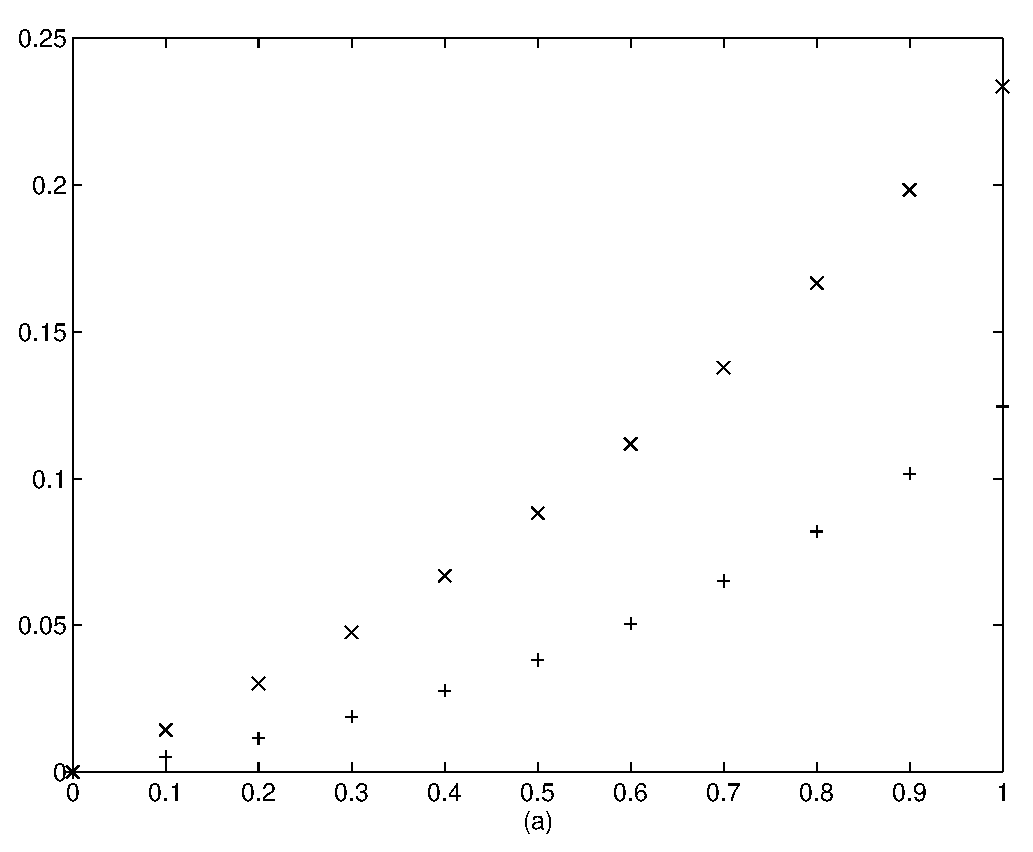
\psfig{file=../figures/globerr1.eps,width=2.9in}
   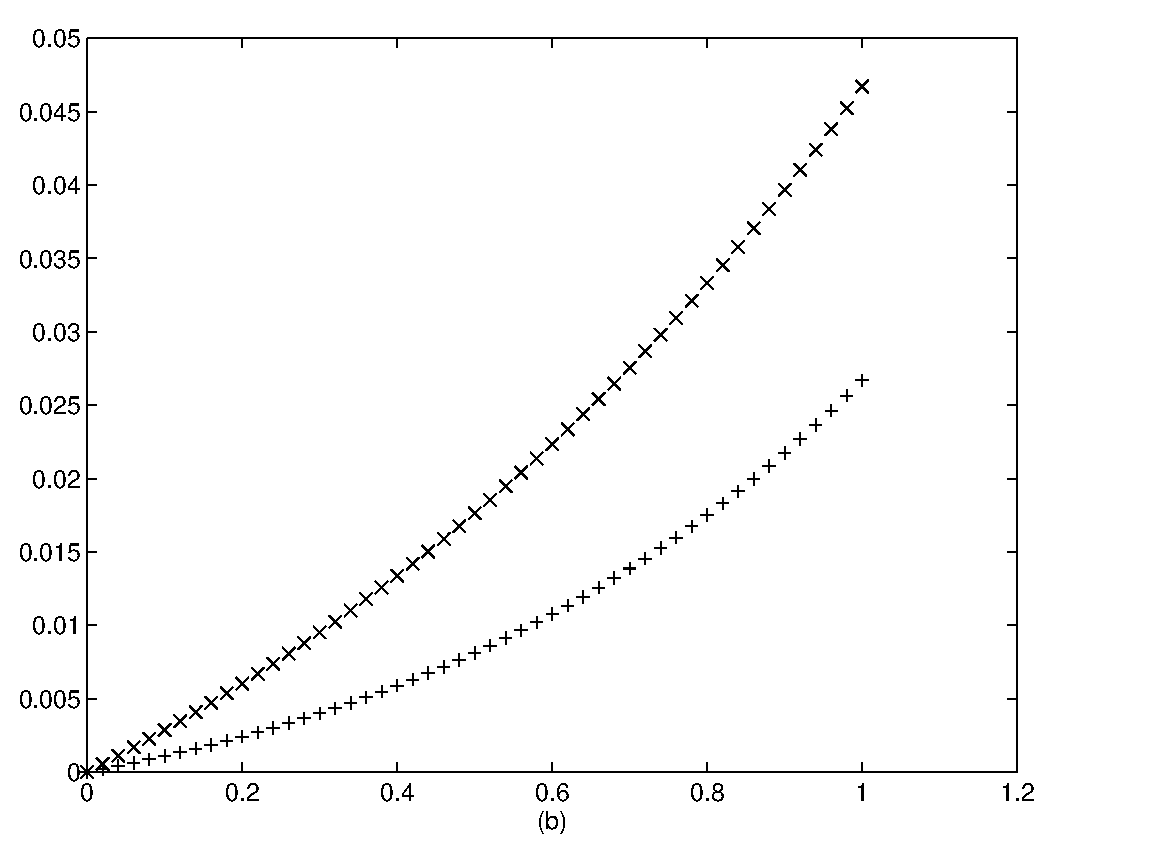
\psfig{file=../figures/globerr2.eps,width=3.3in}}
   \caption{Comparison of the global discretization error (marked by
   $+$) with its estimate given in \protect\eqref{eq:globerr} 
   (marked by $\times$) for the step sizes (a) $h=0.1$ and 
   (b) $h=0.02$.}
   \label{fig:globerr1}
\end{figure*}

\subsubsection*{Explicit Computation of Error Bounds}
\index{error bound!explicit computation}

Another important consequence of Proposition~\ref{prop:globerr1} is
that it allows us to compute the solution of the initial value
problem \eqref{eq:simplest} on a given interval $[0,T]$ up to a
prescribed accuracy.  Indeed, we just have to use the estimate
\eqref{eq:globerr} on the global discretization error.  

For an illustration of this fact suppose that we want to approximate 
a solution of \eqref{eq:simplest} on the interval $t\in [0,2]$
where the maximal global discretization 
error\index{Euler's method!global discretization error} is less than $0.01$.
It follows from \eqref{eq:globerr} that this is certainly the case if the
step size $h$ is chosen such that
\[
e^2(e^2-1)\frac{h}{2} = 0.01,
\]
or, equivalently,
\[
h = \frac{0.02}{e^2(e^2-1)} \approx 0.000424.
\]
Indeed, if this is the case then we find  with \eqref{eq:globerr}
\[
|\epsilon(k)| \le e^2(e^{kh}-1)\frac{h}{2} \le e^2(e^2-1)\frac{h}{2} = 0.01.
\]
The result of the corresponding \Matlab computation of the global
discretization error is shown in Figure~\ref{fig:globerr2}.
\begin{figure}[htb]
   \centerline{%
   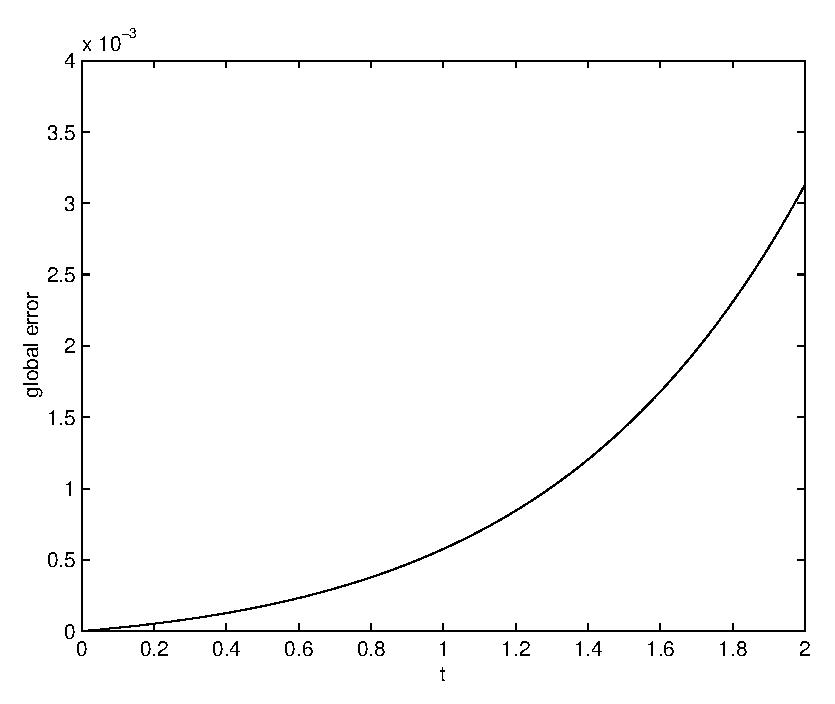
\psfig{file=../figures/globerr5.eps,width=3.6in}}
   \caption{The global discretization error for the solution of
   \protect\eqref{eq:simplest} on the interval $[0,2]$ with
   step size $h=0.000424$.}
   \label{fig:globerr2}
\end{figure}



\EXER

\TEXER

\noindent In Exercises~\ref{c15.2.1a} -- \ref{c15.2.1c} compute
bounds on the local and global error for Euler's method applied
to the given initial value problem.  Perform the same steps as in
the treatment of the initial value problem \eqref{eq:simplest} in
the text.
\begin{exercise} \label{c15.2.1a}
$\frac{\dps dx}{\dps dt} = 3x,\quad x(0)=1$.

\begin{solution}
\ans Local discretization error:
\[
\delta(k+1) \le
e^{3T}\frac{(3h)^2}{2} \quad \mbox{for all $h\ge 0$.}
\]
Global discretization error:
\[
|\epsilon(k)| \le e^{3T}(e^{3T}-1)\frac{3h}{2}.
\]

\soln Euler's method applied to the initial value problem takes the form
\[
\begin{array}{rclcl}
t_{k+1} & = & t_k+h & & \\
x_{k+1} & = & x_k + h 3 x_k & = & (1+3h)x_k
\end{array}
\]
where $k=0,1,\ldots,K-1$.

{\em Local error:} we assume that the
numerical solution is exact up to step $k$, that is,
we start in $x(t_k)=e^{3t_k}$.  Then the local discretization error
$\delta(k+1)$ is given by
\[
\delta(k+1) = x(t_{k+1}) - (x(t_k) + h 3x(t_k))=
e^{3t_{k+1}} - (1+3h)e^{t_k}.
\]
Since $t_k = kh$ we obtain
\[
\delta(k+1) = e^{3t_{k+1}} - (1+3h)e^{t_k} =
e^{3(k+1)h} - (1+3h)e^{3kh} = e^{3kh}(e^{3h}-(1+3h)).
\]
By definition of the exponential function
\[
e^{3h}-(1+3h) = \frac{(3h)^2}{2}+\frac{(3h)^3}{6}+\cdots =
\frac{(3h)^2}{2}\left[ 1+\frac{(3h)}{3}+\frac{(3h)^2}{12}+\cdots\right]
\le \frac{(3h)^2}{2}e^{3h}.
\]
Since $(k+1)h=(k+1)/K\le T$ for $k=0,1,\ldots,K-1$ we finally have the
desired bound on the local discretization error:
\[
\delta(k+1) = e^{3kh}(e^{3h}-(1+3h)) \le
e^{3(k+1)h}\left(\frac{(3h)^2}{2}\right)\le
e^{3T}\frac{(3h)^2}{2} \quad \mbox{for all $h\ge 0$.}
\]

{\em Global error:} we have for $k=1,2,\ldots,K$
\[
x(t_k)=(1+3h)x(t_{k-1})+\delta(k),
\]
and subtracting
\[
x_k = (1+3h)x_{k-1}
\]
leads to
\[
x(t_k) - x_k = (1+3h)(x(t_{k-1})-x_{k-1})+\delta(k).
\]
Therefore
\begin{eqnarray*}
|\epsilon(k)| & = & |x(t_k) - x_k| =
|(1+3h)(x(t_{k-1})-x_{k-1})+\delta(k)|\\
& \le & (1+3h)|\epsilon(k-1)|+\delta_h
\end{eqnarray*}
since
\[
\delta(k)\le \delta_h = e^{3T}\frac{(3h)^2}{2}.
\]
Apply this formula repeatedly until $k$ is zero,
\[
\begin{array}{rcl}
|\epsilon(k)|&\le&(1+3h)|\epsilon(k-1)|+\delta_h\\
&\le& (1+3h)[(1+3h)|\epsilon(k-2)|+\delta_h]+\delta_h\\
&=& (1+3h)^2|\epsilon(k-2)| + ((1+3h) + 1)\delta_h\\
&\le& (1+3h)^2[(1+3h)|\epsilon(k-3)|+\delta_h] + ((1+3h) + 1)\delta_h\\
&=& (1+3h)^3|\epsilon(k-3)| + ((1+3h)^2 + (1+3h) + 1)\delta_h\\
&\vdots& \\
&\le & (1+3h)^k|\epsilon(0)| + ((1+3h)^{k-1} +\cdots + (1+3h) + 1)\delta_h.
\end{array}
\]
Since $\epsilon(0)=x(t_0) - x_0=0$
\[
|\epsilon(k)| \le \frac{(1+3h)^k -1}{3h}\delta_h.
\]
With $1+3h\le e^{3h}$ we have the bound on the global discretization error:
\[
|\epsilon(k)| \le \frac{1}{3h} (e^{3kh}-1)\delta_h=
\frac{1}{3h}(e^{3kh}-1)e^{3T}\frac{(3h)^2}{2} =
e^{3T}(e^{3kh}-1)\frac{3h}{2}
\le e^{3T}(e^{3T}-1)\frac{3h}{2}.
\]

\end{solution}
\end{exercise}
\begin{exercise} \label{c15.2.1b}
$\frac{\dps dx}{\dps dt} = x,\quad x(0)=2$.

\begin{solution}
\ans Local discretization error:
\[
\delta(k+1) \le
2e^{T}\frac{h^2}{2} \quad \mbox{for all $h\ge 0$.}
\]
Global discretization error:
\[
|\epsilon(k)| \le 2e^{T}(e^{T}-1)\frac{h}{2}.
\]

\soln Euler's method applied to the initial value problem takes the form
\[
\begin{array}{rclcl}
t_{k+1} & = & t_k+h & & \\
x_{k+1} & = & x_k + h x_k & = & (1+h)x_k
\end{array}
\]
where $k=0,1,\ldots,K-1$.

{\em Local error:} we assume that the
numerical solution is exact up to step $k$, that is,
we start in $x(t_k)=2e^{t_k}$.  Then the local discretization error
$\delta(k+1)$ is given by
\[
\delta(k+1) = x(t_{k+1}) - (x(t_k) + h x(t_k))=
2e^{t_{k+1}} - (1+h)2e^{t_k}.
\]
Since $t_k = kh$ we obtain
\[
\delta(k+1) = 2e^{t_{k+1}} - (1+h)2e^{t_k} =
2e^{(k+1)h} - (1+h)2e^{kh} = 2e^{kh}(e^{h}-(1+h)).
\]
By definition of the exponential function
\[
e^{h}-(1+h) \le \frac{h^2}{2}e^{h}.
\]
Since $(k+1)h=(k+1)/K\le T$ for $k=0,1,\ldots,K-1$ we finally have the
desired bound on the local discretization error:
\[
\delta(k+1) = 2e^{kh}(e^{h}-(1+h)) \le
2e^{(k+1)h}\left(\frac{h^2}{2}\right)\le
2e^{T}\frac{h^2}{2} \quad \mbox{for all $h\ge 0$.}
\]

{\em Global error:} we have for $k=1,2,\ldots,K$
\[
x(t_k)=(1+h)x(t_{k-1})+\delta(k),
\]
and subtracting
\[
x_k = (1+h)x_{k-1}
\]
leads to
\[
x(t_k) - x_k = (1+h)(x(t_{k-1})-x_{k-1})+\delta(k).
\]
Therefore
\begin{eqnarray*}
|\epsilon(k)| & = & |x(t_k) - x_k| =
|(1+h)(x(t_{k-1})-x_{k-1})+\delta(k)|\\
& \le & (1+h)|\epsilon(k-1)|+\delta_h
\end{eqnarray*}
since
\[
\delta(k)\le \delta_h = 2e^{T}\frac{h^2}{2}.
\]
Apply this formula repeatedly until $k$ is zero,
\[
\begin{array}{rcl}
|\epsilon(k)|&\le&(1+h)|\epsilon(k-1)|+\delta_h\\
&\le& (1+h)[(1+h)|\epsilon(k-2)|+\delta_h]+\delta_h\\
&=& (1+h)^2|\epsilon(k-2)| + ((1+h) + 1)\delta_h\\
&\le& (1+h)^2[(1+h)|\epsilon(k-3)|+\delta_h] + ((1+h) + 1)\delta_h\\
&=& (1+h)^3|\epsilon(k-3)| + ((1+h)^2 + (1+h) + 1)\delta_h\\
&\vdots& \\
&\le & (1+h)^k|\epsilon(0)| + ((1+h)^{k-1} +\cdots + (1+h) + 1)\delta_h.
\end{array}
\]
Since $\epsilon(0)=x(t_0) - x_0=0$
\[
|\epsilon(k)| \le \frac{(1+h)^k -1}{h}\delta_h.
\]
With $1+h\le e^{h}$ we have the bound on the global discretization error:
\[
|\epsilon(k)| \le \frac{1}{h} (e^{kh}-1)\delta_h=
\frac{1}{h}(e^{kh}-1)2e^{T}\frac{h^2}{2} =
2e^{T}(e^{kh}-1)\frac{h}{2}
\le 2e^{T}(e^{T}-1)\frac{h}{2}.
\]


\end{solution}
\end{exercise}
\begin{exercise} \label{c15.2.1c}
$\frac{\dps dx}{\dps dt} = 3x,\quad x(0)=2$.

\begin{solution}
\ans Local discretization error:
\[
\delta(k+1) \le
2e^{3T}\frac{(3h)^2}{2} \quad \mbox{for all $h\ge 0$.}
\]
Global discretization error:
\[
|\epsilon(k)| \le 2e^{3T}(e^{3T}-1)\frac{3h}{2}.
\]

\soln Euler's method applied to the initial value problem takes the form
\[
\begin{array}{rclcl}
t_{k+1} & = & t_k+h & & \\
x_{k+1} & = & x_k + h 3x_k & = & (1+3h)x_k
\end{array}
\]
where $k=0,1,\ldots,K-1$.

{\em Local error:} we assume that the
numerical solution is exact up to step $k$, that is,
we start in $x(t_k)=2e^{3t_k}$.  Then the local discretization error
$\delta(k+1)$ is given by
\[
\delta(k+1) = x(t_{k+1}) - (x(t_k) + h 3 x(t_k))=
2e^{3t_{k+1}} - (1+3h)2e^{3t_k}.
\]
Since $t_k = kh$ we obtain
\[
\delta(k+1) = 2e^{3t_{k+1}} - (1+3h)2e^{3t_k} =
2e^{3(k+1)h} - (1+3h)2e^{3kh} = 2e^{3kh}(e^{3h}-(1+3h)).
\]
By definition of the exponential function
\[
e^{3h}-(1+3h) = \frac{(3h)^2}{2}+\frac{(3h)^3}{6}+\cdots =
\frac{(3h)^2}{2}\left[ 1+\frac{(3h)}{3}+\frac{(3h)^2}{12}+\cdots\right]
\le \frac{(3h)^2}{2}e^{3h}.
\]
Since $(k+1)h=(k+1)/K\le T$ for $k=0,1,\ldots,K-1$ we finally have the
desired bound on the local discretization error:
\[
\delta(k+1) = 2e^{3kh}(e^{3h}-(1+3h)) \le
2e^{3(k+1)h}\left(\frac{(3h)^2}{2}\right)\le
2e^{3T}\frac{(3h)^2}{2} \quad \mbox{for all $h\ge 0$.}
\]

{\em Global error:} we have for $k=1,2,\ldots,K$
\[
x(t_k)=(1+3h)x(t_{k-1})+\delta(k),
\]
and subtracting
\[
x_k = (1+3h)x_{k-1}
\]
leads to
\[
x(t_k) - x_k = (1+3h)(x(t_{k-1})-x_{k-1})+\delta(k).
\]
Therefore
\begin{eqnarray*}
|\epsilon(k)| & = & |x(t_k) - x_k| =
|(1+3h)(x(t_{k-1})-x_{k-1})+\delta(k)|\\
& \le & (1+3h)|\epsilon(k-1)|+\delta_h
\end{eqnarray*}
since
\[
\delta(k)\le \delta_h = 2e^{3T}\frac{(3h)^2}{2}.
\]
Apply this formula repeatedly until $k$ is zero,
\[
\begin{array}{rcl}
|\epsilon(k)|&\le&(1+3h)|\epsilon(k-1)|+\delta_h\\
&\le& (1+3h)[(1+3h)|\epsilon(k-2)|+\delta_h]+\delta_h\\
&=& (1+3h)^2|\epsilon(k-2)| + ((1+3h) + 1)\delta_h\\
&\le& (1+3h)^2[(1+3h)|\epsilon(k-3)|+\delta_h] + ((1+3h) + 1)\delta_h\\
&=& (1+3h)^3|\epsilon(k-3)| + ((1+3h)^2 + (1+3h) + 1)\delta_h\\
&\vdots& \\
&\le & (1+3h)^k|\epsilon(0)| + ((1+3h)^{k-1} +\cdots + (1+3h) + 1)\delta_h.
\end{array}
\]
Since $\epsilon(0)=x(t_0) - x_0=0$
\[
|\epsilon(k)| \le \frac{(1+3h)^k -1}{3h}\delta_h.
\]
With $1+3h\le e^{3h}$ we have the bound on the global discretization error:
\[
|\epsilon(k)| \le \frac{1}{3h} (e^{3kh}-1)\delta_h=
\frac{1}{3h}(e^{3kh}-1)2e^{3T}\frac{(3h)^2}{2} =
2e^{3T}(e^{3kh}-1)\frac{3h}{2}
\le 2e^{3T}(e^{3T}-1)\frac{3h}{2}.
\]

\end{solution}
\end{exercise}

\begin{exercise} \label{c15.2.2}
Apply the implicit Euler method to the initial value problem
\eqref{eq:simplest}.  Then determine a formula for the local 
discretization error that is analogous to \eqref{eq:locerrdef}.
{\bf Hint:} Before proceeding as for Euler's method solve
for $x_{k+1}$ in \eqref{eq:impleulit} in this specific case.

\begin{solution}
\ans Local discretization error:
\[
\delta(k+1) = e^{t_{k+1}} - \frac{1}{1-h} e^{t_k}.
\]

\soln The implicit Euler method applied to the initial value problem
\eqref{eq:simplest} takes the form
\[
\begin{array}{rclc}
t_{k+1} & = & t_k+h & \\
x_{k+1} & = & x_k + h x_{k+1} &
\end{array}
\]
where $k=0,1,\ldots,K-1$.  Solving for $x_{k+1}$ yields
\[
x_{k+1} = \frac{1}{1-h}x_k.
\]
We assume that the numerical solution is exact up to step $k$, that is,
we start in $x(t_k)=e^{t_k}$.  Then the local discretization error
$\delta(k+1)$ is given by
\[
\delta(k+1) = x(t_{k+1}) - \frac{1}{1-h}x(t_k)=
e^{t_{k+1}} - \frac{1}{1-h}e^{t_k}.
\]

\end{solution}
\end{exercise}

\CEXER

\noindent In Exercises~\ref{c15.2.3a} -- \ref{c15.2.3b}
determine a step size $h$ such that the global discretization error
for the solution of \eqref{eq:simplest} on the given interval using 
Euler's method is less than the given absolute tolerance.  Verify 
your results by a computation of the global discretization error 
using \Matlabp.
\begin{exercise} \label{c15.2.3a}
Interval $[0,4]$ and absolute tolerance $2$.

\begin{solution}
\ans $h=0.0014$.

\soln Using the bound on the global discretization error
given in Proposition~\ref{prop:globerr1} we can choose a
step length $h$ satisfying
\[
e^4(e^4-1)\frac{h}{2} = 2,
\]
or, equivalently,
\[
h = \frac{4}{e^4(e^4-1)} \approx 0.0014.
\]
Now $4/h \approx 2927$, and we can verify our result using the
following \Matlab commands:
\begin{verbatim}
h      = 0.0014;
t(1)   = 0;
x(1)   = 1;
err(1) = 0;
est(1) = 0;
K      = 2927;
for k = 1:K
    t(k+1) = t(k)+h;
    x(k+1) = (1+h)*x(k);
  err(k+1) = exp(t(k+1))-x(k+1);
end
plot(t,err)
xlabel('t')
ylabel('global error')
\end{verbatim}
Indeed, by this choice of $h$ the error is always smaller than $0.18$.


\end{solution}
\end{exercise}
\begin{exercise} \label{c15.2.3b}
Interval $[0,5]$ and absolute tolerance $10$.

\begin{solution}
\ans $h=0.000914$.

\soln Using the bound on the global discretization error
given in Proposition~\ref{prop:globerr1} we can choose a
step length $h$ satisfying
\[
e^{5}(e^{5}-1)\frac{h}{2} = 10,
\]
or, equivalently,
\[
h = \frac{20}{e^{5}(e^{5}-1)} \approx 0.000914.
\]
Now $5/h \approx 5470$, and we can verify our result using the
following \Matlab commands:
\begin{verbatim}
h      = 0.000914;
t(1)   = 0;
x(1)   = 1;
err(1) = 0;
est(1) = 0;
K      = 5470;
for k = 1:K
    t(k+1) = t(k)+h;
    x(k+1) = (1+h)*x(k);
  err(k+1) = exp(t(k+1))-x(k+1);
end
plot(t,err)
xlabel('t')
ylabel('global error')
\end{verbatim}
Indeed, by this choice of $h$ the error is always smaller than $0.35$.


\end{solution}
\end{exercise}

\begin{exercise} \label{c15.2.4}
Suppose that you want to solve \eqref{eq:simplest} by Euler's
method with a fixed step size $h=0.005$ on the interval $[0,T]$.  
How large can you choose $T$ so that the global discretization
error does not exceed $0.05$?  Confirm your result using \Matlabp.

\begin{solution}
\ans $T=1.609$.

\soln Using the bound on the global discretization error
given in Proposition~\ref{prop:globerr1} we can choose
$T$ satisfying
\[
e^{T}(e^{T}-1)\frac{0.005}{2} = 0.05,
\]
or, equivalently,
\[
e^{2T} - e^T - 20 = 0.
\]
Solving this quadratic equation in $e^T$ leads to the positive
solution
\[
e^T = 5 \Rightarrow T \approx 1.609.
\]
Now $T/h \approx 321$, and we can verify our result using the
following \Matlab commands:
\begin{verbatim}
h      = 0.005;
t(1)   = 0;
x(1)   = 1;
err(1) = 0;
est(1) = 0;
K      = 321;
for k = 1:K
    t(k+1) = t(k)+h;
    x(k+1) = (1+h)*x(k);
  err(k+1) = exp(t(k+1))-x(k+1);
end
plot(t,err)
xlabel('t')
ylabel('global error')
\end{verbatim}
Indeed, by this choice of $T$ the error is smaller than $0.02$.




\end{solution}
\end{exercise}

\end{document}
